
\documentclass[portrait,10pt, a4paper]{article}
\usepackage[margin=0.3in]{geometry}
\usepackage[utf8]{inputenc}
\usepackage{multicol}

\usepackage{mathtools}
\usepackage{tikz}
\usepackage{ifthen}

\begin{document}
\raggedright
\begin{multicols*}{3}
\section{Introduction}
\subsection{What is an algorithm?}
Formally, an algorithm is just a procedure to turn one form of input into another one.

\subsection{The champion problem}
		Given a set of n elements, how do we select the minimum or the maximum ones? The \textit{naive}
		solution involves performing a linear scan on all the items in the array. However, for each item in the 
		array, we would need to perform some amount of computation. Thus, the time it takes to solve the problem
		would scale as the size of the input scales up.

\subsection{Selection Sort}	
		Given a set of n elements, output the entire sequence in non-decreasing order. Using the champion problem,
		we see that that we can \textit{reduce} the sorting problem to the champion problem. We pull the min number
		from the unsorted section of the array, and insert it into the sorted prefix array. Since we pull the minimum
		number from $n$, then $n-1$ elements, then we will pull the elements in a non-decreasing order.

		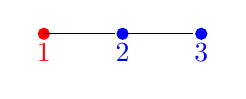
\begin{tikzpicture}
				\filldraw[red](-1,0) circle (2pt) node[anchor=north]{1};
				\draw[black, thin] (-1,0) -- (-.1,0);
				\filldraw[blue](0,0) circle (2pt) node[anchor=north]{2};
				\draw[black, thin] (0,0) -- (.9, 0);
				\filldraw[blue] (1,0) circle (2pt) node[anchor=north]{3};
		\end{tikzpicture}

		During the first call to $\text{champion}(i,n)$, we get the smallest value and swap it with the first item of a 
		sorted array. Repeating this process eventually gives us the correct answer.
\subsection{Insertion Sort}
		This is similar to the way we sort a deck of cards. For card $i$, we move from position $i$, until we find the 
		previous item that is less than the number.
\subsection{Asymptotic notation}
		When we talk about how many calculations some operation takes, we mean to say \textit{how the number of calculations		} scale with the size of the input. We can assign a formula for the amount of calculations, then we take the leading
		exponent, and call  it the complexity. We classify it into several portions:

		\[ f(n) \leq C \times g(n) \forall n \geq n_{0}\]
		
		Thus, if a function $f(n)$ is $O(n)$, then $f(n)$ varies from $g(n)$ by no less than a constant factor. This makes
		it easier to discuss the \textit{time-complexity}.
\subsection{Merge Sort}
		The main idea is that we have two different arrays, and we want to just compare item $j$ and item $i$ for every
		one in the two arrays. Using this way, we then recursively sort the two halves of each subarray until we hget all
		the base cases. This then gives us an algo with $O(n\log(n))$.

\subsection{Recurrence Relations}
		We can describe the way how the instances realte to previoius instances of the problem. There are several methods:
		The substitution method, where we unroll the loop; the Recursion-tree method, where we guess an draw the 
		recursion tree method; the final one is the Master Theorem.
\section{Lower Bounds}
		\subsection{Membership Query Problem}	
			Basically, we want to know whether for a given array x with $n$ elements, there exists an $x$ and $i$ such 	
			that $A[i] = x$. The naive solution involves a \textit{linear scan}. If the array is sorted, then we can 
			sort the array in $O\log(n)$ with \textit{Binary Search}. Within the comparison-based model, the ordering
			between the elements can only be determined with comparisons.
		\subsection{More Asymptotic Notation}
			After we learned $O(n)$, we define $\Omega(n)$ and $\Theta(n)$, which act as a lower and upper bound,
			respectively.

			After that, we introduce $o(n)$ and $\omega(n)$, which are defined as:
			\[ \lim_{x\to\infty}\frac{f(n)}{g(n)} = 0\] and 
			\[ \lim_{x\to\infty}\frac{f(n)}{g(n)} = \infty\]
				
			You want to remember: \textbf{if $f(n)=o(g(n)),\text{then} f(n)=O(g(n))$, but not-vice-versa}. Use L'Hopital's
			rule to show this is sometimes easier to do.

			\textbf{asymptotically optimal:} When an algorithm runs in $\Omega(f(n))$ and $O(f(n))$, we know that the 
			algorithm can't be improved by a \textit{superconstant} factor.
		\subsection{Sorting Lower Bound}
			So far, we have a limit of $\Omega(n\log(n))$ for the comparison-based model, becuase both its upper bound and
			lower bound estimates are the same. If we can choose one of the $n!$ permutations, we shold then ask the 
			evil adversary to remove  a certain number of the possible permutations based on the ordering of the elements.
			We can show that $n\log(n)$ is asymptotically optimal.
\section{Divide and Conquer}
	\subsection{What exactly is D\&C?}
		D\&C  involves recursion, or solving the same problem for a smaller instance of the problem. The idea is 
		that to solve a problem of size $n$, we need the solutions to smaller instances of the problem and then 
		somehow merge them together (i.e. the conquer step). In the mergesort this would be merging the two
		arrays after they have been sorted for lower instances of the problem.
	\subsection{Quick Sort}
		This algo chooses a \textit{pivot} from the array (different ways of choosing it), then creates two arrays
		, $S$ and $L$. In $S$ we place all the elements less than $k$(our pivot), and in $L$ the elements larger.
		We then recursively call the function on these two arrays.

		What is the running time? It depends on the relative sizes of S and L. If either is always empty, then
		we will just be recursing on $(n-1)$ every time, which will lead to $O(n^{2})$. If $|S|-|L|<1$, then our 
		recursion is \textit{balanced} and thus reaches the desired $O(n\log(n))$ time.

		However, for a arbitrary ratio  $|S|:|L|$, the worst-case is $(n,n-1,...,1)$, so $O(n^{2})$
	\subsection{Randomized Quick Sort}
		Random selections of pivots usually result in balanced trees. Why? By the \textit{Chernov Inquality}, we
		know that a bounded portion of the values will be a larger distance away from the mean.
	\subsection{Selection}
		AKA the $k-th$ order statistics, we seek to find the index of the k-th smallest number. We can split
		the arrays into $S$ and $L$ again, and if 
\section{Linear-Time Algorithms}
	\subsection{Seelction}
		The naive way to find the min element is to do a linear scan. How to find the order statistic in linear 
		time? It depends on the selection of a good pivot. 
\section{Geometric Problems}
	\subsection{Bichromatic Planar Matching}
		Given  a set of $n$ points on a plane, we want to find a pairing of points such that we can draw lines 
		to all of them without them crossing.

		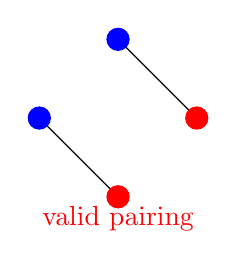
\begin{tikzpicture}
				\draw[black, thin] (-1,0) -- (0,-1);
				\draw[black, thin] (0,1) -- (1,0);
				\filldraw[blue] (0,1) circle (4pt) ;
				\filldraw[blue] (-1,0) circle (4pt);
				\filldraw[red] (1,0) circle (4pt);	
				\filldraw[red] (0,-1) circle (4pt) node[anchor=north]{valid pairing};	
		\end{tikzpicture}
			
		Notice how neither line crosses when connecting to the other points. Generalizing to $n$ points, no lines
		should intersect when trying to find one such pairing. A possible solution: assign an arbitrary 
		arrangement and individually fix it.
\end{multicols*}
\end{document}
